\documentclass{beamer}
\usepackage{graphicx}
\usetheme{boxes}  %% Themenwahl
\usecolortheme{dolphin}
\setbeamertemplate{footline}[page number]{}
\setbeamertemplate{navigation symbols}{}

\title{Videobrick \\ Open Hardware project \\ 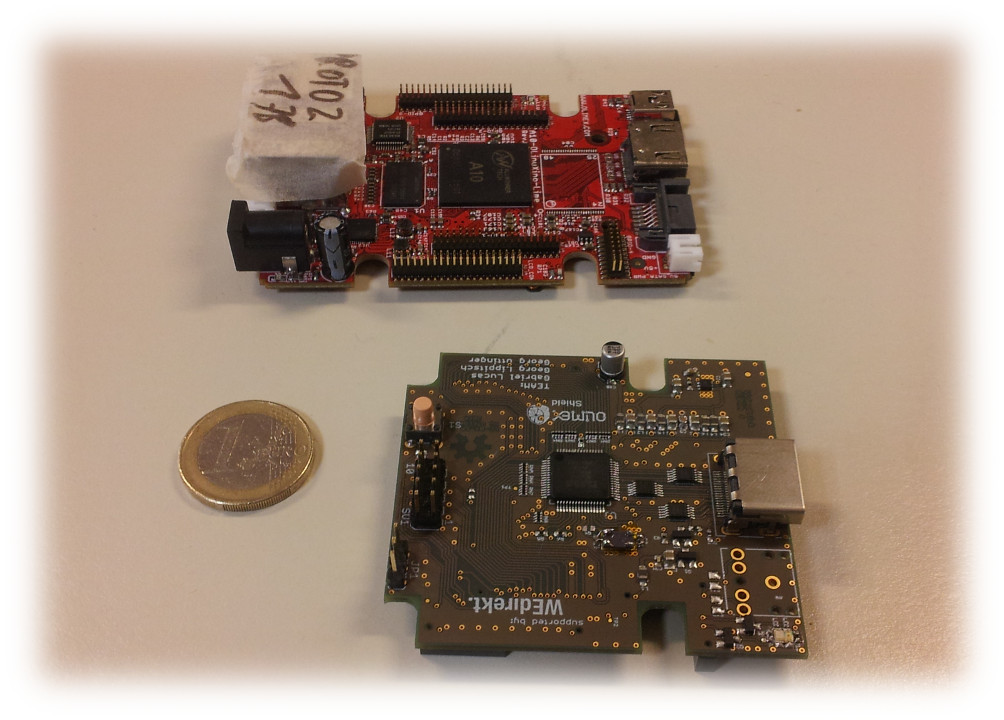
\includegraphics[width=160px]{title.jpg}}
\author{Georg Lippitsch}
\date{\today}
 
\begin{document}
\maketitle
 
\begin{frame} %%Eine Folie

  \frametitle{What is it?} %%Folientitel
  Open Hardware embedded ARM board with HDMI video/audio input.

  \begin{center}
    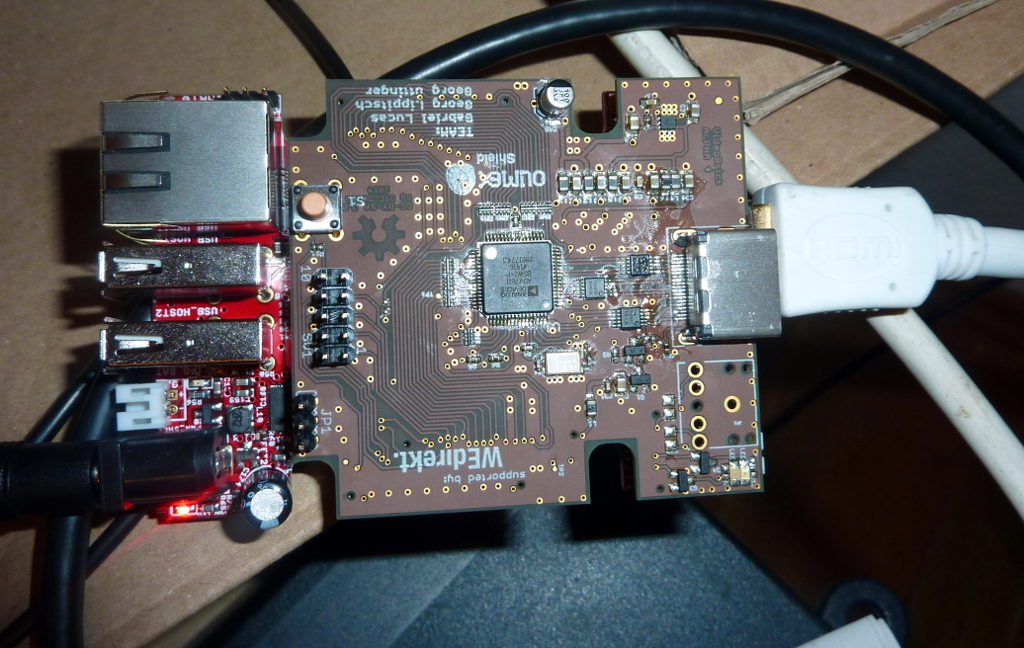
\includegraphics[width=120px]{vbrick.jpg}
  \end{center}

  \begin{block}{Goal}
    Have a small device to record / encode / stream / whatever from an HDMI sourcce using GStreamer.
  \end{block}

  \begin{block}{Why HDMI?}
    \begin{itemize}
    \item On many video cameras, it's the only video output
    \item Most popular interface for uncompressed digital video
    \end{itemize}
  \end{block}

\end{frame}

\begin{frame} %%Eine Folie

  \frametitle{Olimex OLinuXino}

  \begin{center}
    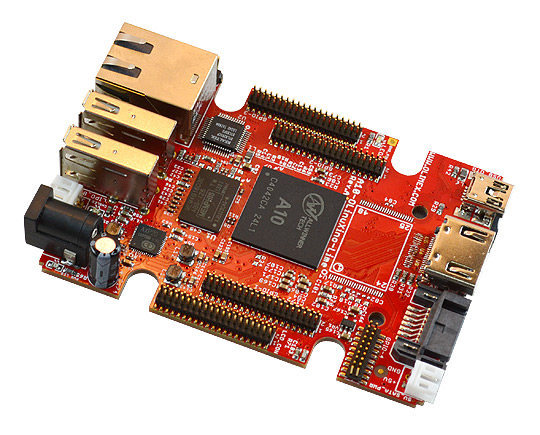
\includegraphics[width=120px]{A10-OLinuXino-LIME-1.jpg}
  \end{center}

  \begin{itemize}
  \item Allwinner A10 or A20 SOC (ARM Cortex A8 or A7)
  \item H.264 encoder
  \item Ethernet
  \item SATA
  \item Open Hardware (Cadsoft Eagle schematics / PC layout available)
  \item From 30 to 55 EUR
  \end{itemize}

\end{frame}

\begin{frame} %%Eine Folie

  \frametitle{HDMI shield}

  \begin{center}
    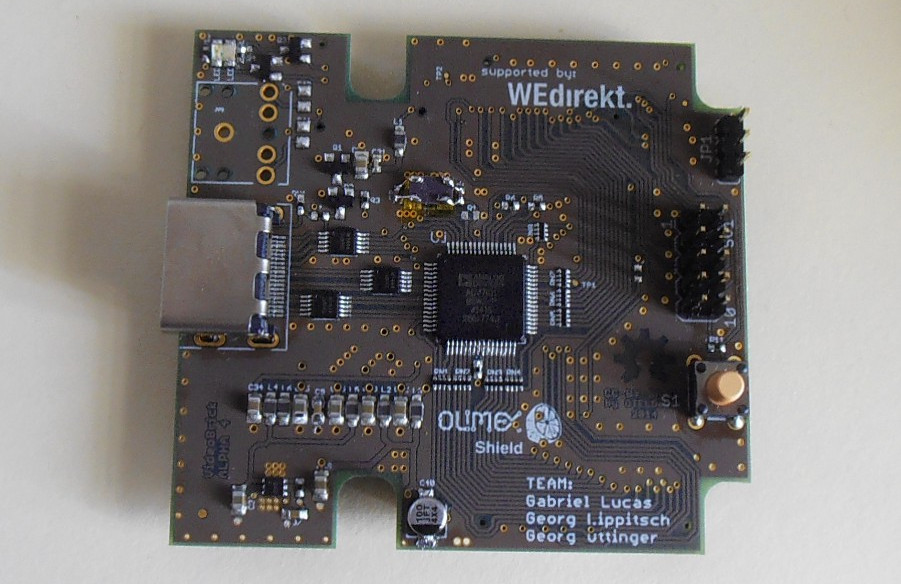
\includegraphics[width=120px]{shield.jpg}
  \end{center}

  \begin{itemize}
  \item Based on Analog Devices ADV7611
  \item Converts HDMI to 24 bit parallel + clock + hsync/vsync
  \item Connected to Allwinner A10/A20 CSI
  \item Open Hardware (Eagle files available, KiCad work in progress)
  \end{itemize}

  \begin{center}
    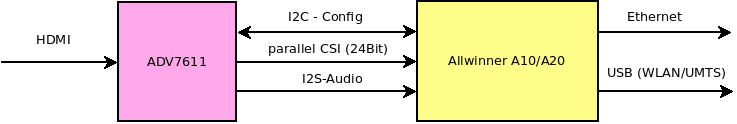
\includegraphics[width=\textwidth]{adv7611_a10.png}
  \end{center}

\end{frame}

\begin{frame} %%Eine Folie

  \frametitle{Current task: Write software}
  \begin{itemize}
  \item We can communicate with ADV7611 via I$^2$C, get a signal out of it
  \item Currently everything is low level kernel hacking, everything in kernel space
  \item We expect to be able to access some video buffer from userspace soon
  \end{itemize}

  \begin{center}
    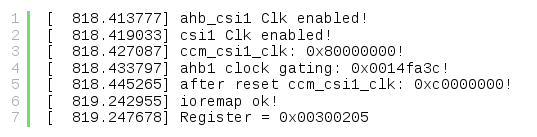
\includegraphics[width=240px]{dmesg.png}
  \end{center}

\end{frame}

\begin{frame} %%Eine Folie

  \frametitle{TODO}
  \begin{itemize}
  \item V4l2 kernel module
  \item GStreamer video source plug-in which can pass parameters to ADV7611
  \item What else?
  \end{itemize}

\end{frame}

\begin{frame} %%Eine Folie

  \frametitle{Schematics}
  \begin{center}
    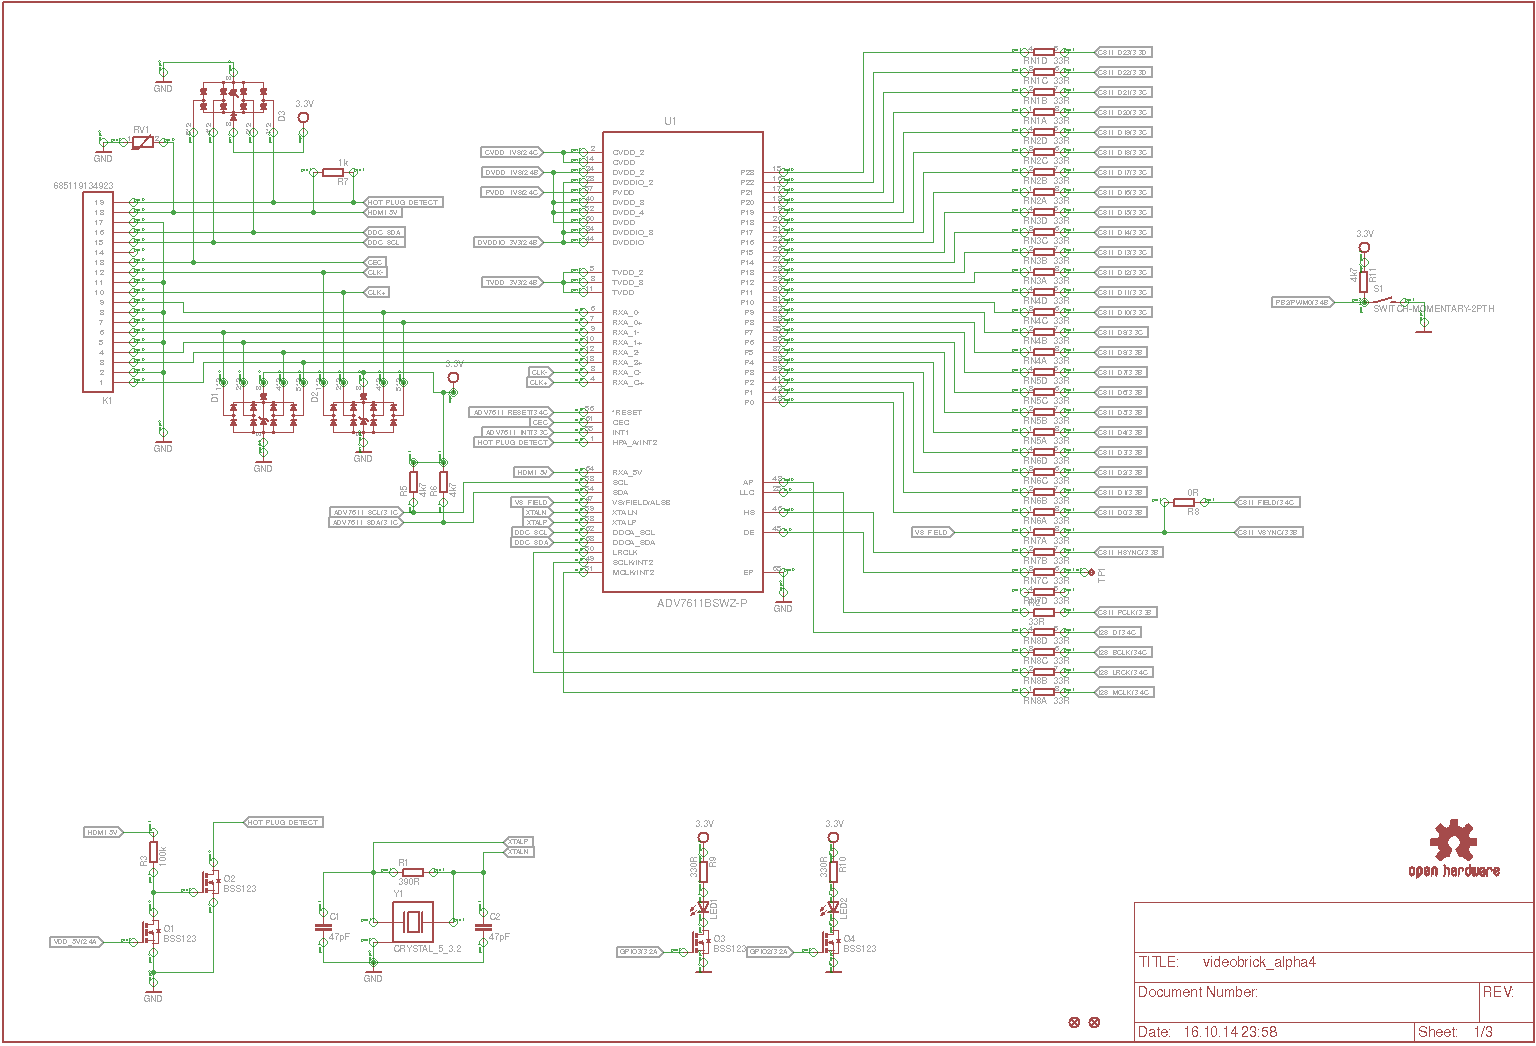
\includegraphics[width=\textwidth]{videobrick_sch.png}
  \end{center}

\end{frame}

\begin{frame} %%Eine Folie

  \frametitle{PC layout}
  \begin{center}
    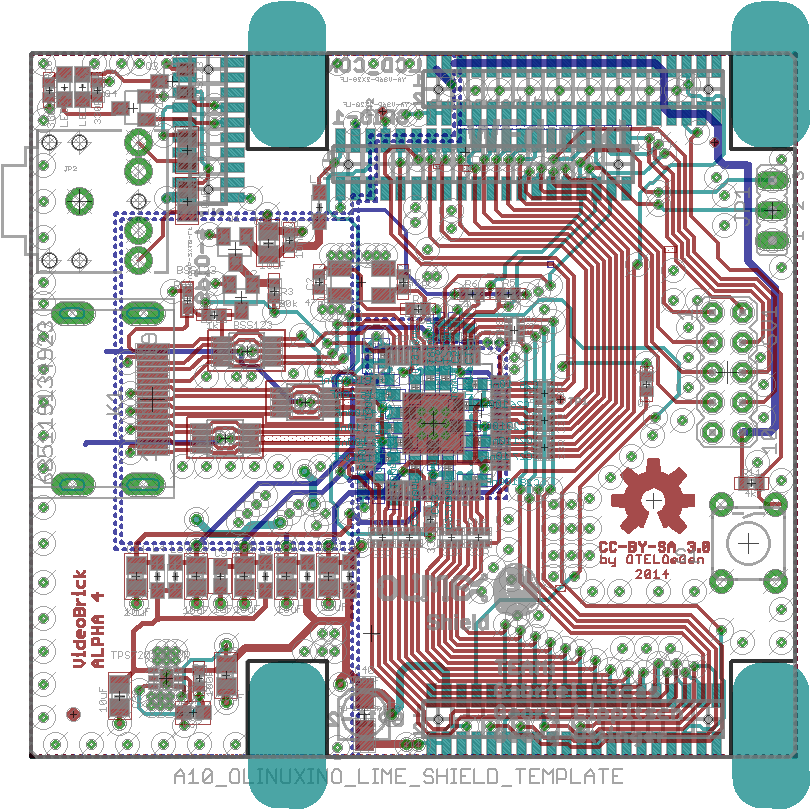
\includegraphics[width=240px]{videobrick_pcb.png}
  \end{center}

\end{frame}

\begin{frame} %%Eine Folie

  \frametitle{Part placement}
  \begin{center}
    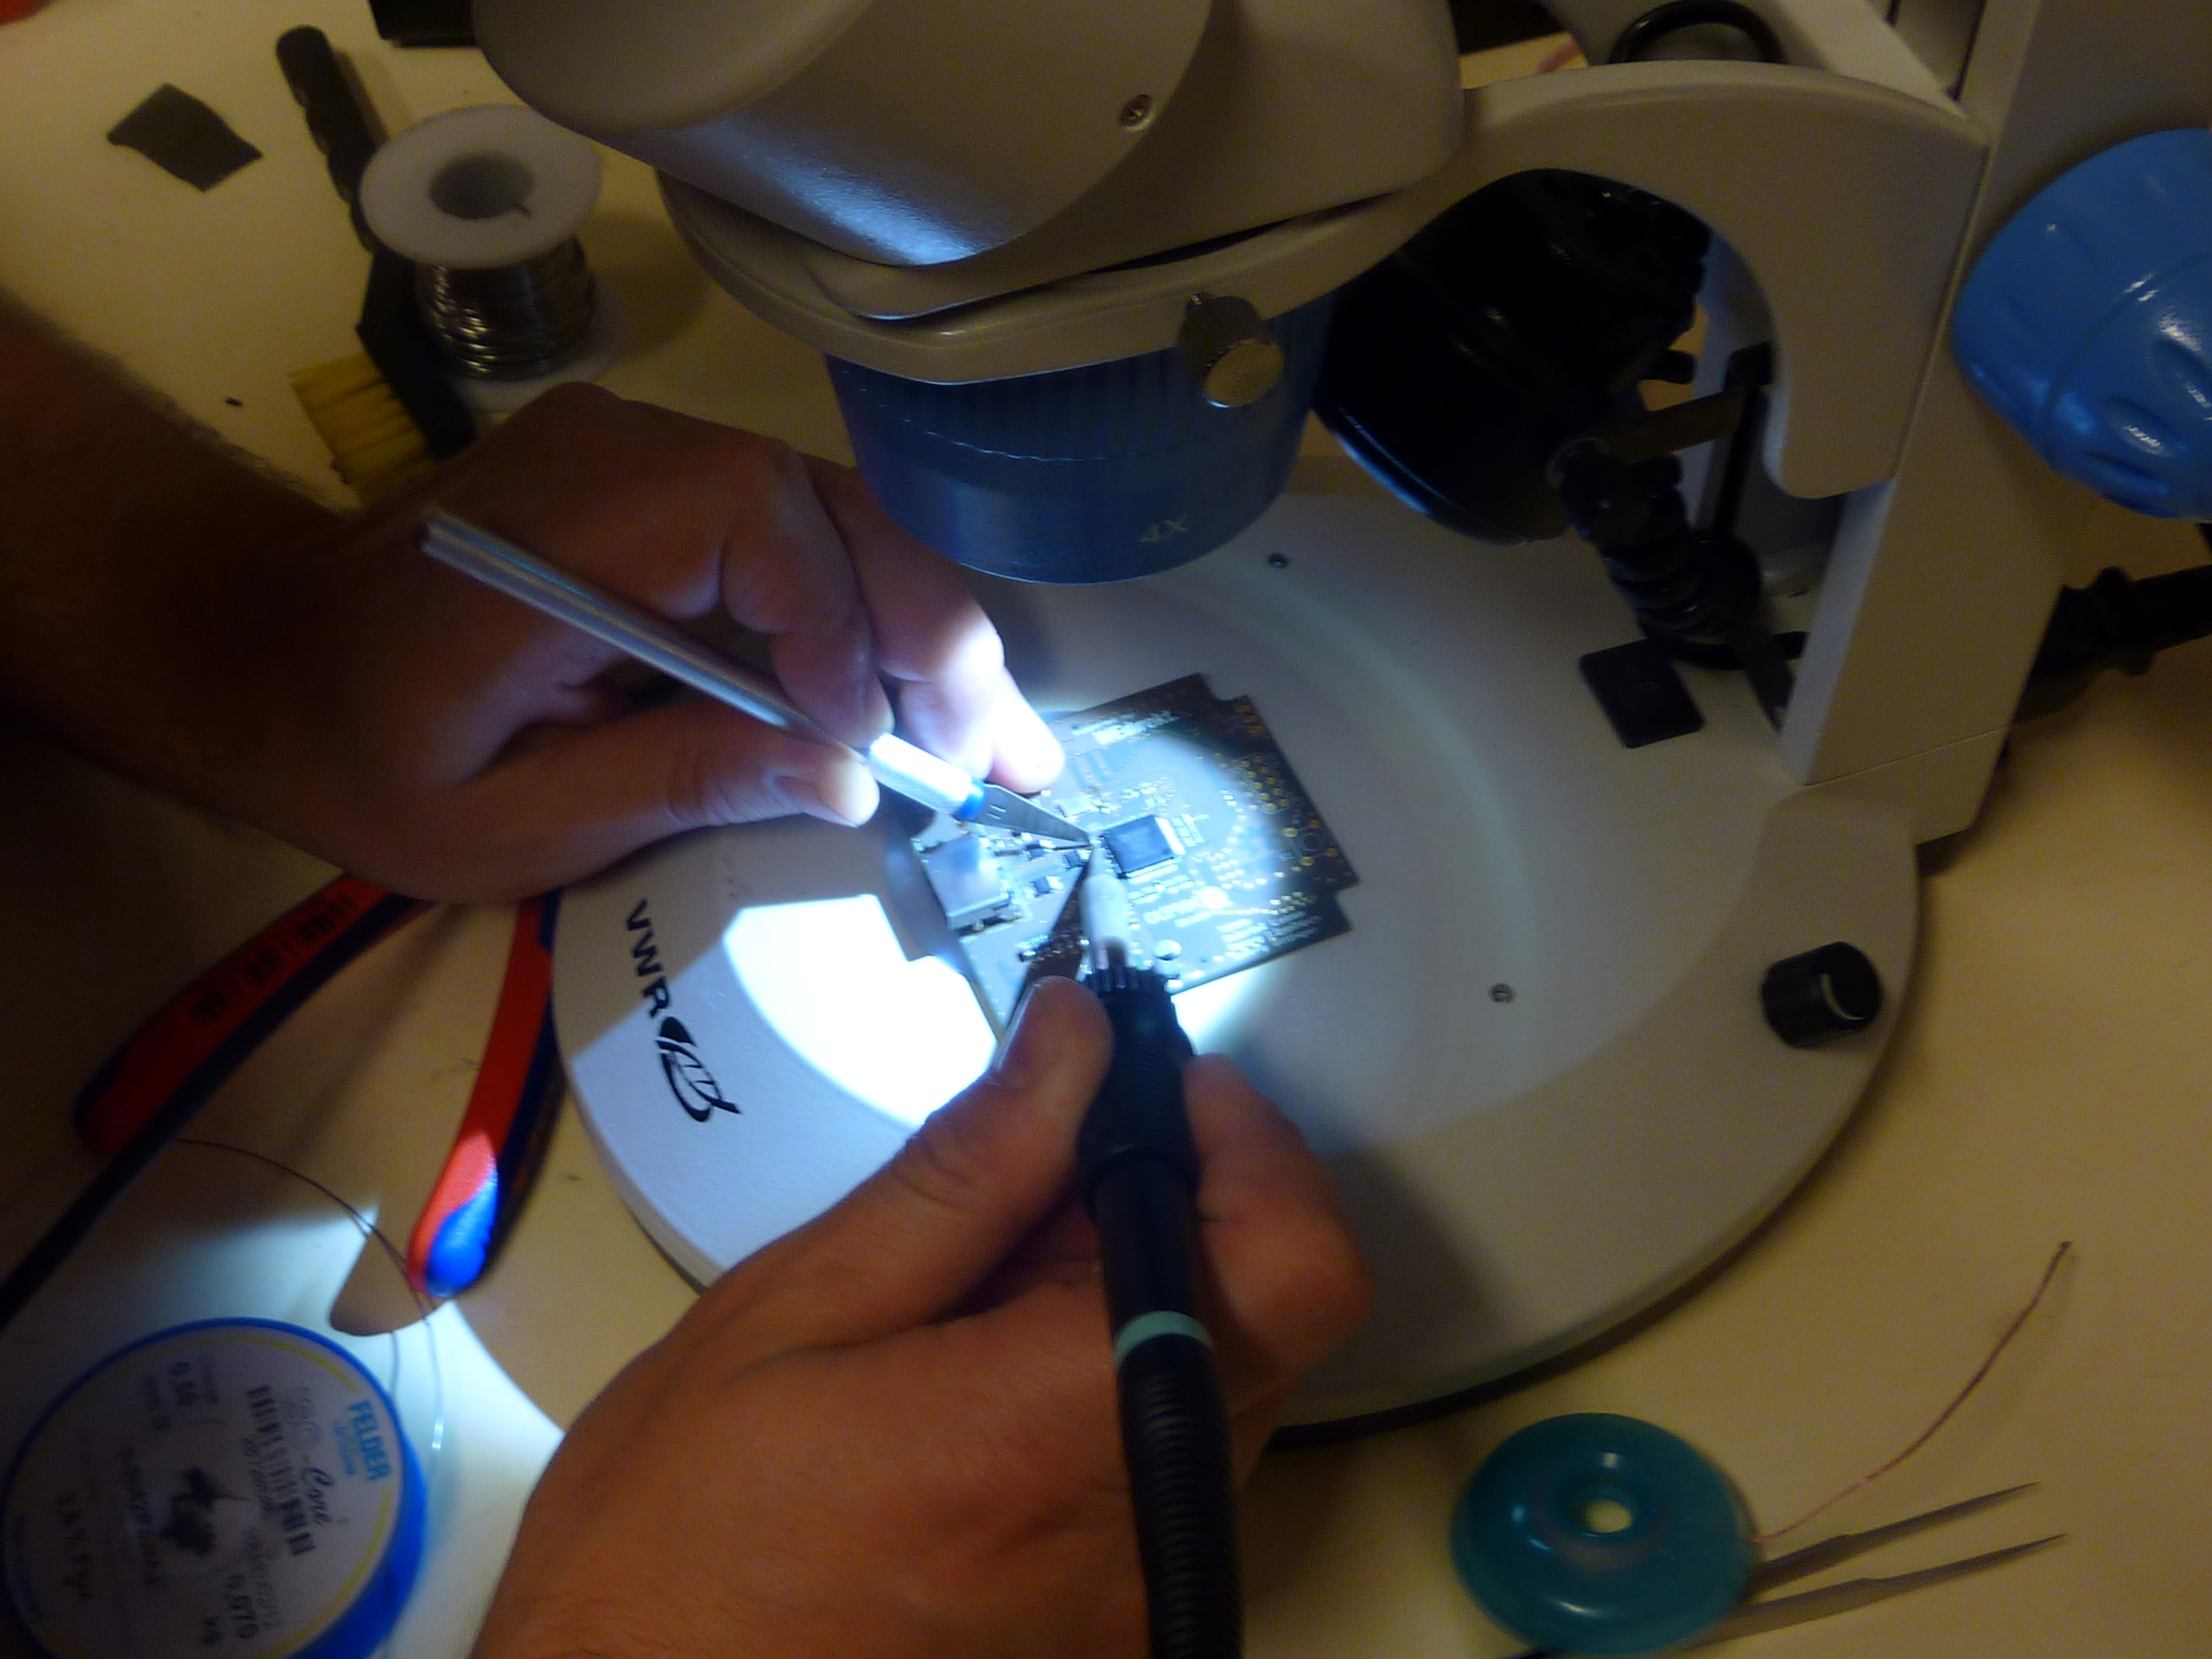
\includegraphics[width=240px]{microscope.jpg}
  \end{center}

\end{frame}

\begin{frame} %%Eine Folie

  \frametitle{Reflow soldering}
  \begin{center}
    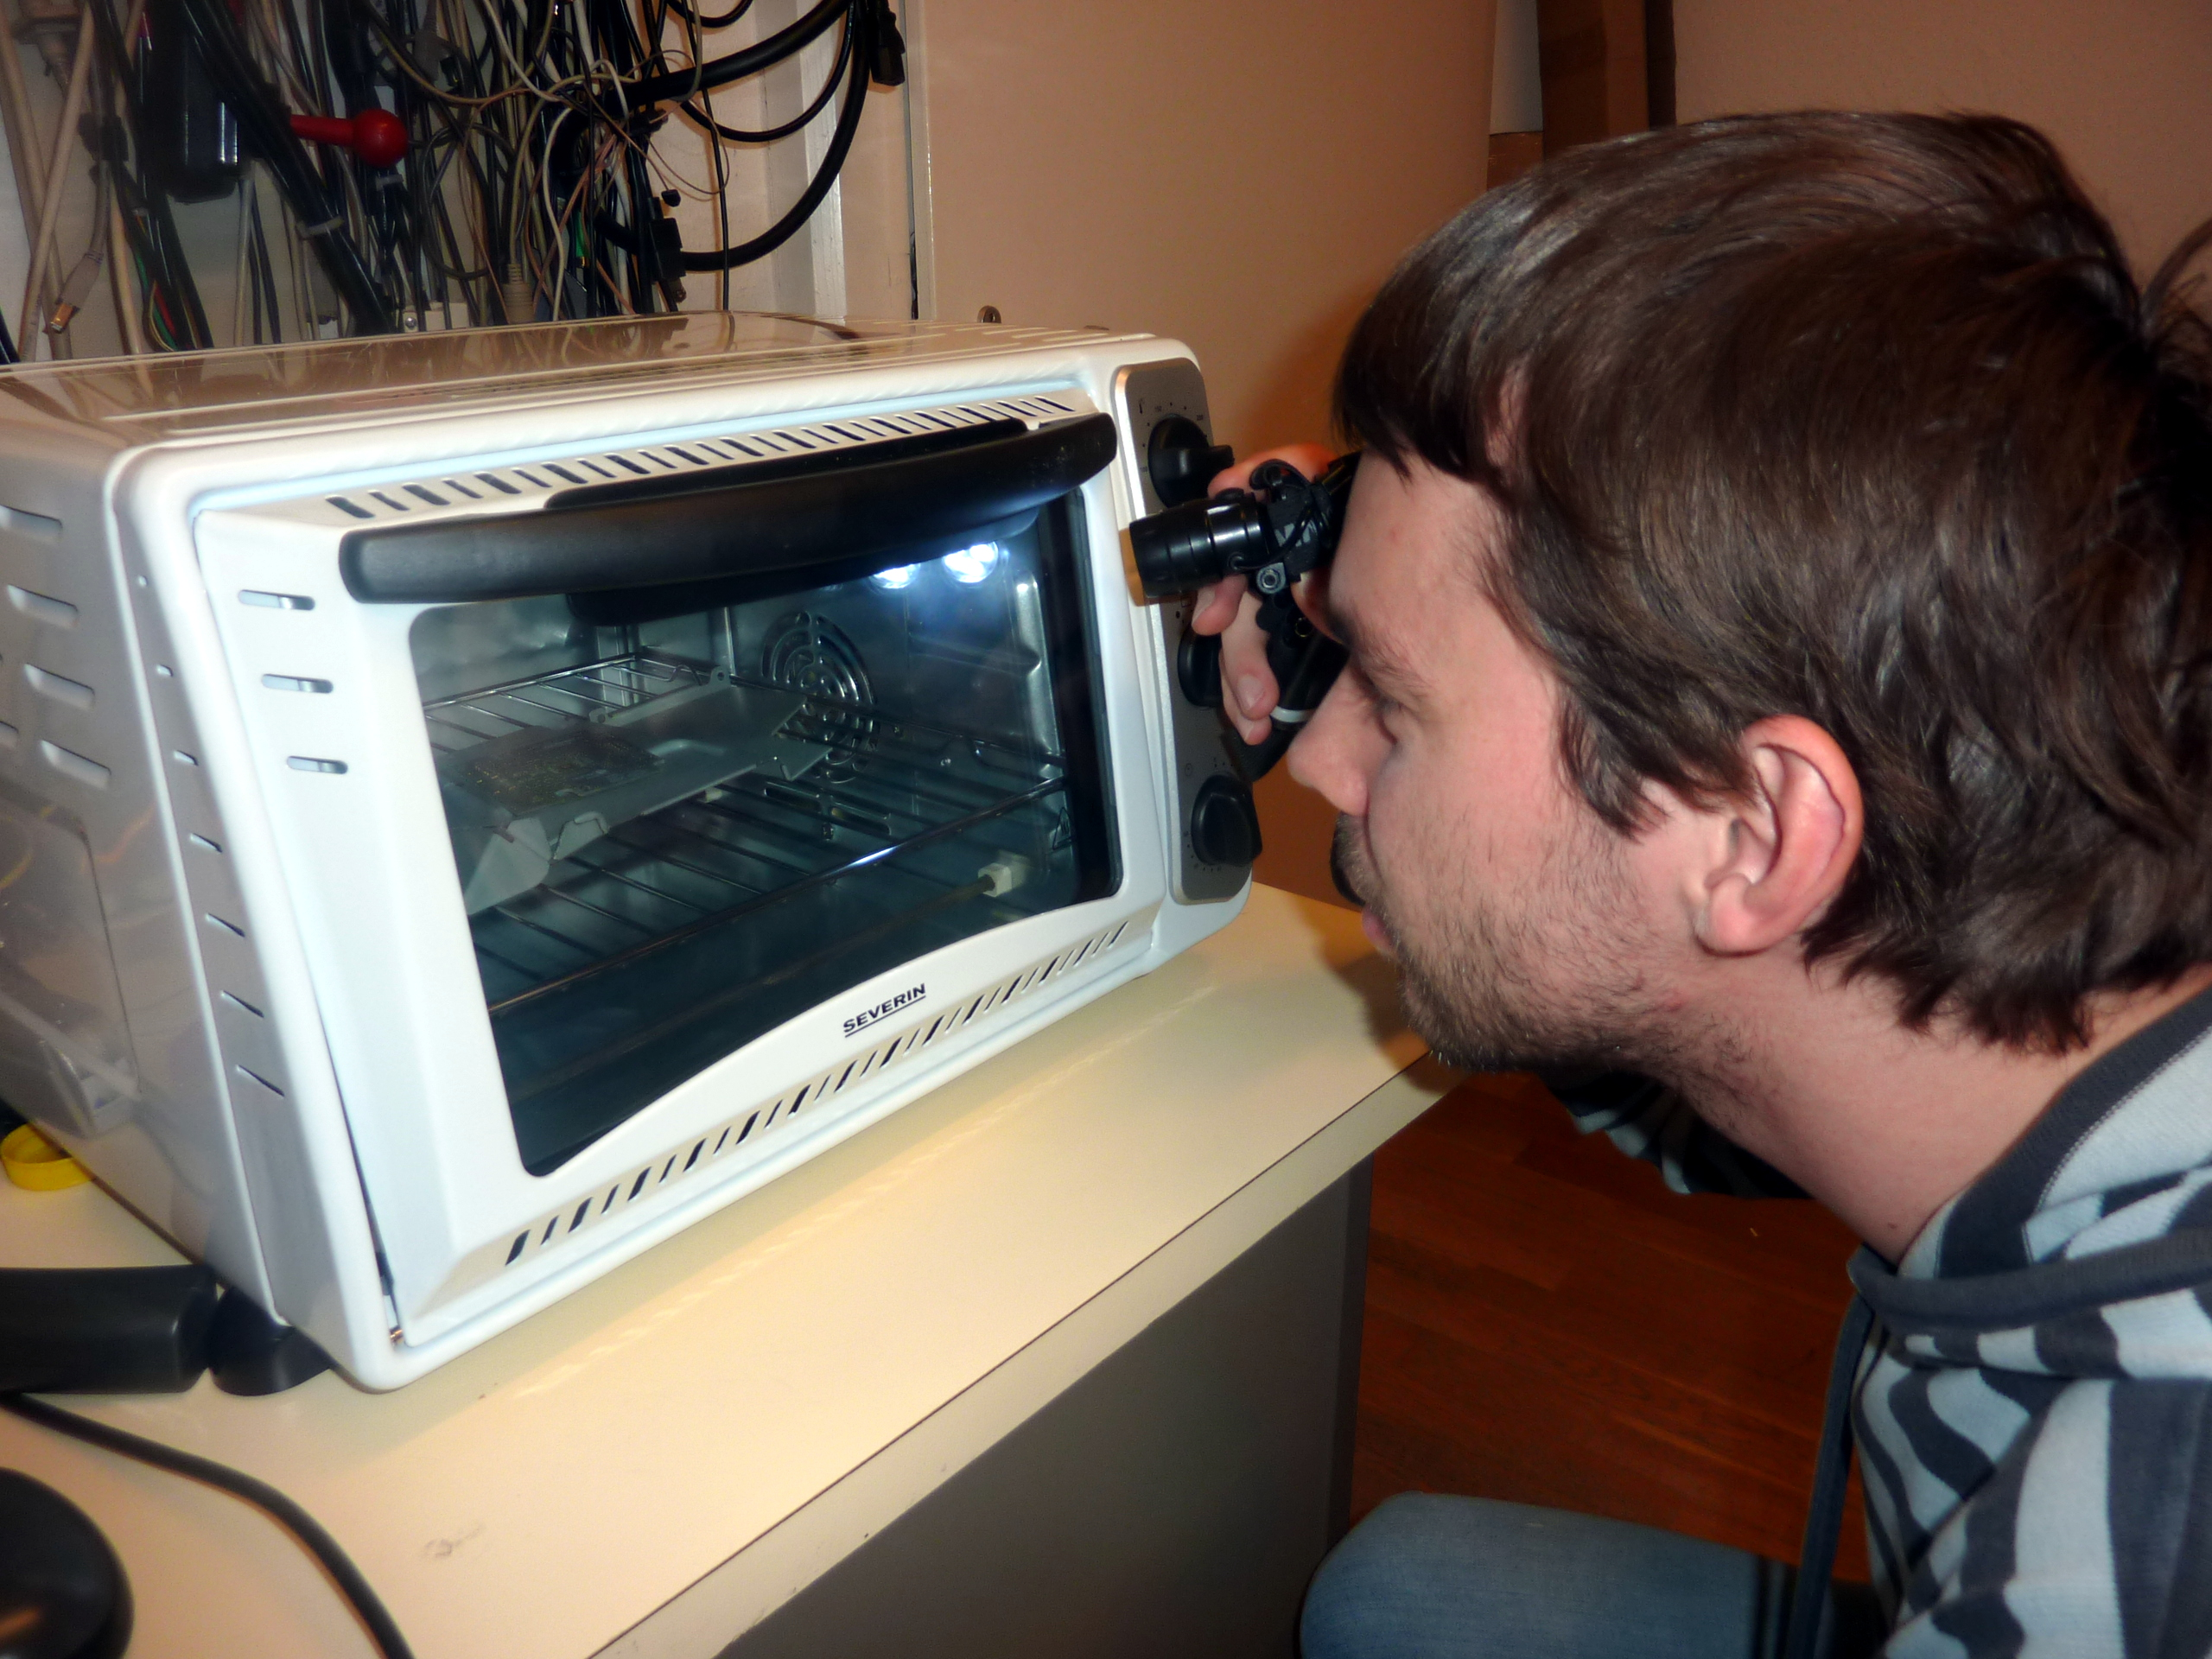
\includegraphics[width=240px]{soldering.jpg}
  \end{center}

\end{frame}

\begin{frame} %%Eine Folie

  \frametitle{Final shield}
  \begin{center}
    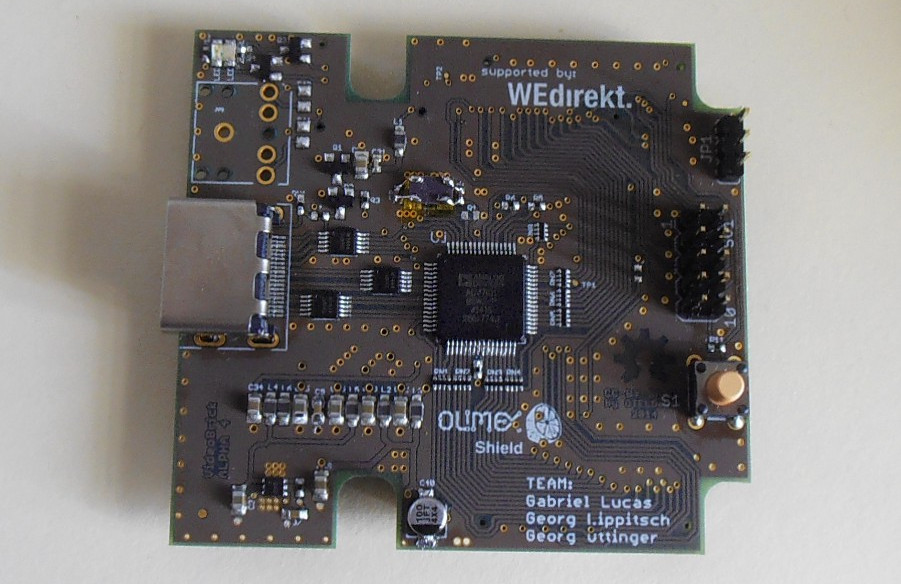
\includegraphics[width=240px]{shield.jpg}
  \end{center}

\end{frame}

\begin{frame} %%Eine Folie
  \frametitle{Please contact us!}

  \begin{center}
    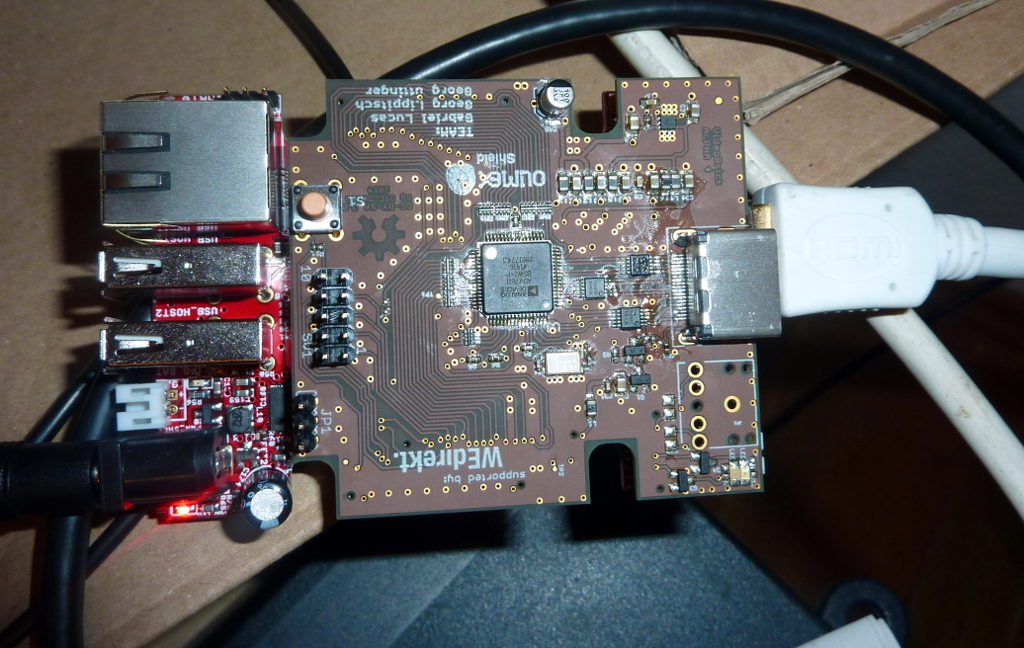
\includegraphics[width=240px]{vbrick.jpg}
  \end{center}

  http://videobrick.wordpress.com/

  http://github.com/videobrick

  georg.lippitsch@gmx.at
\end{frame}

\end{document}
